\section{Introduction}\label{introduction}

\begin{frame}{Basic Analyses}

\center
\textbf{Basic Analyses}: The analyses taught in the first stats course
\vspace{12pt}

\columnsbegin

\begin{column}{0.48\textwidth}
   These include:
   \begin{enumerate}
   \item T-tests
   \item ANOVA
   \item Linear Regression
   \end{enumerate}
   These allow us to assess relationships like that in the figure.
\end{column}\begin{column}{0.48\textwidth}
    \begin{center}
     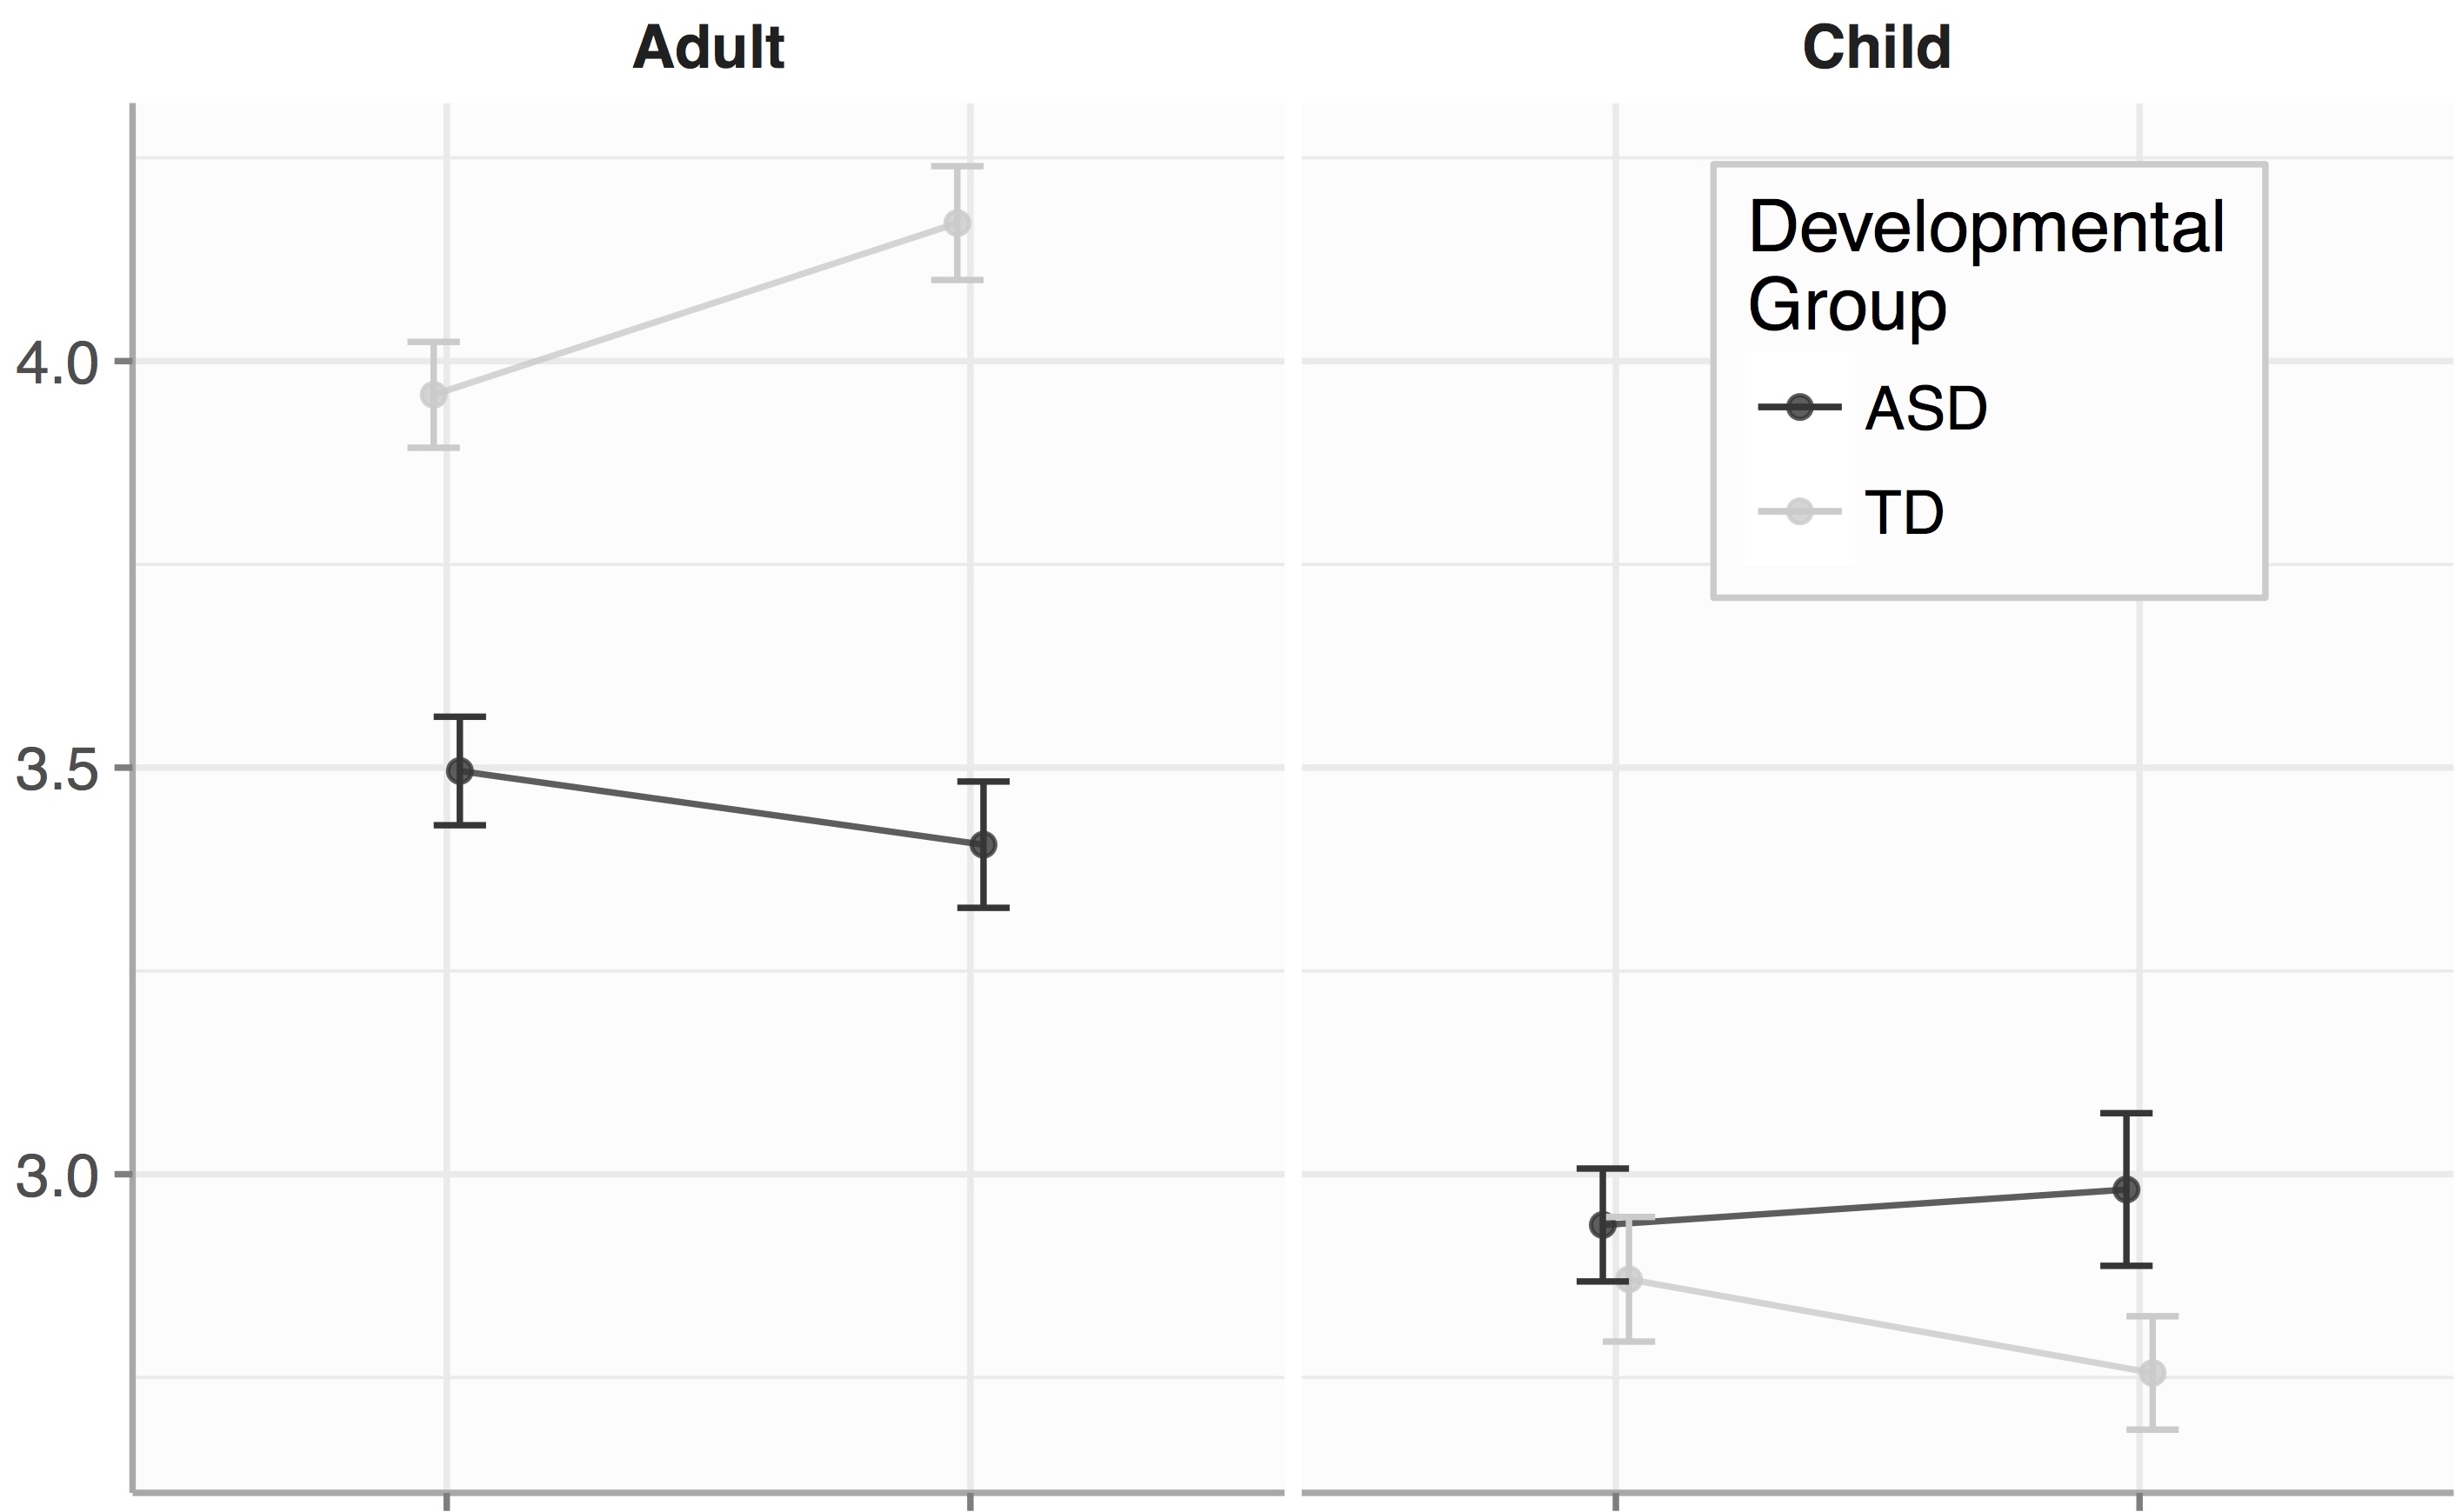
\includegraphics[width=\textwidth]{Figures/FigureInteraction.jpg}
     \end{center}
\end{column}

\columnsend

\vspace{12pt} Maybe surprising:\textbackslash{} These all are doing
essentially the same thing!

First, \textbf{T-TESTS!}

\end{frame}

\section{T-tests}\label{t-tests}

\begin{frame}{Three Types}

\Huge

\begin{enumerate}
\item Simple
\item Independent Samples
\item Paired Samples
\end{enumerate}

\end{frame}

\begin{frame}[fragile]{Three Types}

\Large
Each will be demonstrated using:

\normalsize

\begin{Shaded}
\begin{Highlighting}[]
\NormalTok{df <-}\StringTok{ }\KeywordTok{data.frame}\NormalTok{(}\StringTok{"A"}\NormalTok{=}\KeywordTok{sample}\NormalTok{(}\KeywordTok{c}\NormalTok{(}\DecValTok{0}\NormalTok{,}\DecValTok{1}\NormalTok{), }\DecValTok{100}\NormalTok{, }\DataTypeTok{replace =} \OtherTok{TRUE}\NormalTok{),}
                 \StringTok{"B"}\NormalTok{=}\KeywordTok{rnorm}\NormalTok{(}\DecValTok{100}\NormalTok{),}
                 \StringTok{"C"}\NormalTok{=}\KeywordTok{rnorm}\NormalTok{(}\DecValTok{100}\NormalTok{))}
\NormalTok{df}
\end{Highlighting}
\end{Shaded}

\begin{verbatim}
    A            B            C
1   1 -1.634569035  1.136084564
2   0  0.920975586 -0.351869884
3   1 -0.968021229 -0.339548892
4   1  1.303420399 -0.644911064
5   0  0.439410726 -0.648788673
6   0 -1.117808884  0.324842056
7   1  0.721734088 -0.323065810
8   1  1.718606636 -0.820410249
9   0 -0.371234569 -0.856676250
10  1 -0.178326127 -0.462412105
11  0  1.083850523 -0.161392807
12  0 -0.289617587 -0.960796089
13  1 -0.246831805  0.845917152
14  1 -0.081613180  0.800125540
15  1 -1.536930383  1.171891782
16  1 -0.684215978 -0.229046621
17  1  1.231543422  0.526870953
18  0  0.563204234 -0.314323072
19  1  0.171397001  0.814591067
20  1 -0.311264287  1.315855740
21  1 -0.403534882 -0.906541580
22  0  0.351610044 -0.872218777
23  1 -0.338576212  0.343023629
24  1  0.312558970 -0.204162465
25  0 -0.585202035  1.395629550
26  1 -1.049410156  0.481284824
27  1  0.079897097  2.352618458
28  0  0.439791495  1.372213931
29  1 -0.002278415  0.017997197
30  0  1.637284601  0.051525464
31  0 -0.469598313 -1.963017662
32  0  0.497096978  2.128192635
33  1 -0.521395107  0.136289135
34  1  0.824174338 -1.246384840
35  0  0.330988803 -0.437061252
36  1  1.262561094  1.152622681
37  1  0.335292345 -1.268220397
38  1  1.269723566  0.034905956
39  1  0.260004383 -0.460436462
40  0 -1.117057850 -0.708436846
41  1  2.851912788  2.167531657
42  1 -0.370313058 -1.085693237
43  1  0.038200105  0.928901659
44  1  0.177700462  0.211710557
45  1 -0.101481022 -0.944868711
46  0 -1.666694777 -0.915141686
47  0  0.942609232  1.319975538
48  0  0.990106974 -0.446212612
49  0  0.146141936 -1.108386961
50  1 -0.473292084 -1.024947746
51  1  0.850217266  0.322259396
52  0 -1.583062186  0.778478325
53  1 -0.394951012 -0.310155232
54  0 -0.706960259 -0.347190707
55  1 -0.792216566 -0.172128607
56  1  0.497100157 -0.536517744
57  1 -1.191934034 -0.033037335
58  0  0.238864916  0.962950961
59  1  1.298548476  0.543443542
60  0  0.020674989 -0.306736151
61  1  0.565802080  0.006887048
62  1 -0.860090495 -0.430855810
63  1 -0.709041771 -0.970573527
64  1 -1.382706060  0.578499073
65  0 -0.023300665 -0.588814569
66  0  1.454953468 -1.806758966
67  0 -1.729329714  0.493658797
68  1  0.465471219 -0.277110255
69  0  1.319336324 -0.733826951
70  1 -1.013390999 -1.315215776
71  1  0.440109376  0.539444300
72  0 -1.026394392 -0.040152954
73  1  0.222982423 -0.074825223
74  0  0.176055822 -0.647127692
75  0  0.398564958  2.139666185
76  0  1.158115503  1.306449146
77  1  0.989228685  1.976198873
78  1 -0.828132017 -0.723377216
79  1  0.156833670 -0.931352031
80  1 -1.533376430  0.431705255
81  1  0.154717833  0.834249825
82  1  1.470925335  0.384222847
83  0  0.262567969 -0.731864900
84  0  0.300999745 -0.500317146
85  1  0.002254230 -0.441152703
86  0 -0.735631005 -0.631034543
87  0  0.567250168  0.524560828
88  0  1.583581144  1.476513837
89  1  0.729729554 -0.713471902
90  1  1.173136623 -0.256999513
91  0  0.350464656 -1.061639714
92  0 -0.470193063  1.171594211
93  0 -0.182501537  0.418581773
94  0  1.789376664 -0.851301255
95  0 -1.526278546  1.749740755
96  1 -0.324492286  0.481482878
97  1 -1.488347705  1.934347450
98  0 -0.415240223 -1.004758464
99  1  0.620589880  0.319392143
100 0 -0.910278021 -0.459085326
\end{verbatim}

\end{frame}

\begin{frame}[fragile]{Simple}

\center
Comparing a mean of a variable with \(\mu\).

\begin{Shaded}
\begin{Highlighting}[]
\KeywordTok{t.test}\NormalTok{(df}\OperatorTok{$}\NormalTok{B, }\DataTypeTok{mu =} \DecValTok{0}\NormalTok{)}
\end{Highlighting}
\end{Shaded}

\begin{verbatim}

    One Sample t-test

data:  df$B
t = 0.62805, df = 99, p-value = 0.5314
alternative hypothesis: true mean is not equal to 0
95 percent confidence interval:
 -0.1255241  0.2417868
sample estimates:
 mean of x 
0.05813135 
\end{verbatim}

\end{frame}

\begin{frame}[fragile]{Independent Samples}

\center
Comparing the means of two groups (\texttt{dfA} is the grouping
variable).

\begin{Shaded}
\begin{Highlighting}[]
\KeywordTok{t.test}\NormalTok{(df}\OperatorTok{$}\NormalTok{B }\OperatorTok{~}\StringTok{ }\NormalTok{df}\OperatorTok{$}\NormalTok{A)}
\end{Highlighting}
\end{Shaded}

\begin{verbatim}

    Welch Two Sample t-test

data:  df$B by df$A
t = 0.1167, df = 90.352, p-value = 0.9074
alternative hypothesis: true difference in means is not equal to 0
95 percent confidence interval:
 -0.3515987  0.3954865
sample estimates:
mean in group 0 mean in group 1 
     0.07063939      0.04869546 
\end{verbatim}

\end{frame}

\begin{frame}[fragile]{Paired Samples}

\center
Comparing repeated measures (e.g., Pretest vs.~Posttest).

\begin{Shaded}
\begin{Highlighting}[]
\KeywordTok{t.test}\NormalTok{(df}\OperatorTok{$}\NormalTok{B, df}\OperatorTok{$}\NormalTok{C, }\DataTypeTok{paired =} \OtherTok{TRUE}\NormalTok{)}
\end{Highlighting}
\end{Shaded}

\begin{verbatim}

    Paired t-test

data:  df$B and df$C
t = 0.15378, df = 99, p-value = 0.8781
alternative hypothesis: true difference in means is not equal to 0
95 percent confidence interval:
 -0.2393093  0.2795205
sample estimates:
mean of the differences 
             0.02010561 
\end{verbatim}

\end{frame}

\begin{frame}[fragile]{Testing Assumptions of T-Tests}

T-tests require that the data be normally distributed with approximately
the same variance.

\begin{Shaded}
\begin{Highlighting}[]
\NormalTok{## Normality}
\KeywordTok{par}\NormalTok{(}\DataTypeTok{mfrow =} \KeywordTok{c}\NormalTok{(}\DecValTok{1}\NormalTok{,}\DecValTok{2}\NormalTok{))}
\KeywordTok{hist}\NormalTok{(df}\OperatorTok{$}\NormalTok{B)}
\KeywordTok{qqnorm}\NormalTok{(df}\OperatorTok{$}\NormalTok{B)}
\KeywordTok{abline}\NormalTok{(}\DataTypeTok{a=}\DecValTok{0}\NormalTok{, }\DataTypeTok{b=}\DecValTok{1}\NormalTok{)}
\end{Highlighting}
\end{Shaded}

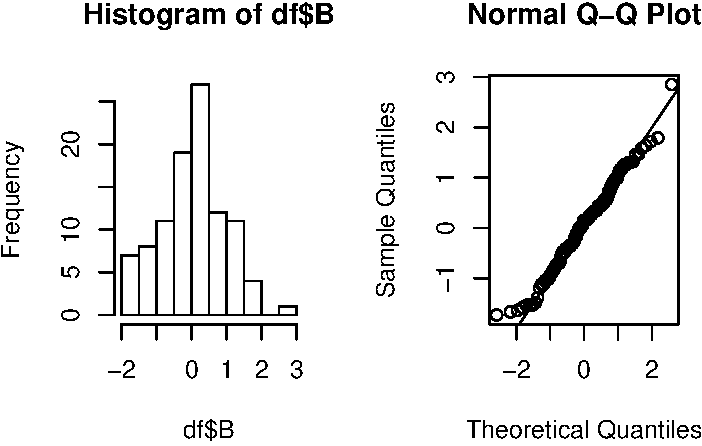
\includegraphics{04_BasicAnalyses_files/figure-beamer/unnamed-chunk-5-1.pdf}

\begin{Shaded}
\begin{Highlighting}[]
\NormalTok{## Variance}
\KeywordTok{var}\NormalTok{(df}\OperatorTok{$}\NormalTok{B)}
\end{Highlighting}
\end{Shaded}

\begin{verbatim}
[1] 0.856701
\end{verbatim}

\begin{Shaded}
\begin{Highlighting}[]
\KeywordTok{var}\NormalTok{(df}\OperatorTok{$}\NormalTok{C)}
\end{Highlighting}
\end{Shaded}

\begin{verbatim}
[1] 0.8903875
\end{verbatim}

\end{frame}

\section{ANOVA}\label{anova}

\begin{frame}[fragile]{Analysis of Variance}

The Analysis of Variance (ANOVA) is highly related to t-tests but can
handle 2+ groups.

\begin{enumerate}
\def\labelenumi{\arabic{enumi}.}
\tightlist
\item
  Provides the same p-value as t-tests
\item
  \(t^2\) = \(F\)
\end{enumerate}

For example:

\begin{Shaded}
\begin{Highlighting}[]
\NormalTok{fit_ano =}\StringTok{ }\KeywordTok{aov}\NormalTok{(df}\OperatorTok{$}\NormalTok{B }\OperatorTok{~}\StringTok{ }\NormalTok{df}\OperatorTok{$}\NormalTok{A)}
\KeywordTok{summary}\NormalTok{(fit_ano)}
\end{Highlighting}
\end{Shaded}

\begin{verbatim}
            Df Sum Sq Mean Sq F value Pr(>F)
df$A         1   0.01  0.0118   0.014  0.907
Residuals   98  84.80  0.8653               
\end{verbatim}

\begin{Shaded}
\begin{Highlighting}[]
\KeywordTok{t.test}\NormalTok{(df}\OperatorTok{$}\NormalTok{B }\OperatorTok{~}\StringTok{ }\NormalTok{df}\OperatorTok{$}\NormalTok{A)}\OperatorTok{$}\NormalTok{p.value}
\end{Highlighting}
\end{Shaded}

\begin{verbatim}
[1] 0.9073553
\end{verbatim}

\end{frame}

\begin{frame}[fragile]{Analysis of Variance}

\begin{Shaded}
\begin{Highlighting}[]
\NormalTok{fit_ano =}\StringTok{ }\KeywordTok{aov}\NormalTok{(df}\OperatorTok{$}\NormalTok{B }\OperatorTok{~}\StringTok{ }\NormalTok{df}\OperatorTok{$}\NormalTok{A)}
\KeywordTok{summary}\NormalTok{(fit_ano)}
\KeywordTok{t.test}\NormalTok{(df}\OperatorTok{$}\NormalTok{B }\OperatorTok{~}\StringTok{ }\NormalTok{df}\OperatorTok{$}\NormalTok{A)}\OperatorTok{$}\NormalTok{p.value}
\end{Highlighting}
\end{Shaded}

Notice in the code:

\begin{itemize}
\tightlist
\item
  We assigned the \texttt{aov()} the name \texttt{fit\_ano} (which we
  could have called anything)
\item
  We used the \texttt{summary()} function to see the F and p values.
\item
  We pulled the p-value right out of the \texttt{t.test()} function.
\end{itemize}

\end{frame}

\begin{frame}{Types}

\huge

\begin{enumerate}
\item One-Way
\item Two-Way (Factorial)
\item Repeated Measures
\item A combination of Factorial and Repeated Measures
\end{enumerate}

\end{frame}

\begin{frame}[fragile]{Types}

We will use the following data set for the examples:

\begin{Shaded}
\begin{Highlighting}[]
\KeywordTok{library}\NormalTok{(tidyverse)}
\NormalTok{df <-}\StringTok{ }\KeywordTok{data.frame}\NormalTok{(}\StringTok{"A"}\NormalTok{=}\KeywordTok{sample}\NormalTok{(}\KeywordTok{c}\NormalTok{(}\DecValTok{0}\NormalTok{,}\DecValTok{1}\NormalTok{), }\DecValTok{100}\NormalTok{, }\DataTypeTok{replace =} \OtherTok{TRUE}\NormalTok{) }\OperatorTok\StringTok{ }\NormalTok{factor,}
                 \StringTok{"B"}\NormalTok{=}\KeywordTok{rnorm}\NormalTok{(}\DecValTok{100}\NormalTok{),}
                 \StringTok{"C"}\NormalTok{=}\KeywordTok{rnorm}\NormalTok{(}\DecValTok{100}\NormalTok{),}
                 \StringTok{"D"}\NormalTok{=}\KeywordTok{sample}\NormalTok{(}\KeywordTok{c}\NormalTok{(}\DecValTok{1}\OperatorTok{:}\DecValTok{4}\NormalTok{), }\DecValTok{100}\NormalTok{, }\DataTypeTok{replace =} \OtherTok{TRUE}\NormalTok{) }\OperatorTok\StringTok{ }\NormalTok{factor)}
\NormalTok{df}
\end{Highlighting}
\end{Shaded}

\begin{verbatim}
    A            B            C D
1   1 -0.765813349 -1.227246676 2
2   1 -1.470818479 -0.953798870 3
3   0  0.318140483  0.676365198 1
4   0  0.478931301 -0.690003721 4
5   1  0.797005962  0.471830539 4
6   0 -1.905408725 -0.241857264 1
7   0  0.369894344 -0.078830706 4
8   0 -0.134437900  0.427207160 4
9   1  0.362070251 -0.213651719 4
10  1  0.265915049  1.024300723 4
11  1 -0.946613034  1.125235666 3
12  0 -0.466031103 -1.058434306 1
13  1 -0.867925709 -1.069450524 3
14  0 -1.909842684  1.948093343 3
15  1 -1.810176148 -1.079491775 2
16  1 -0.033046477 -0.257085609 2
17  0 -2.129897281  0.259753575 2
18  0  0.827970101 -0.098947925 1
19  1  0.869239633  0.648107166 2
20  1 -0.102785100  0.227678141 1
21  0 -0.928487980  0.675733311 2
22  1  1.490281916  1.403217200 4
23  1 -0.178116047  0.184275881 4
24  0 -0.925520103 -0.790497143 1
25  0 -1.424828732  0.431099370 2
26  0  1.600898705 -0.184224468 1
27  0  0.711361021  1.053313443 2
28  0  1.610425832 -0.965543066 4
29  1 -1.234744313  0.037524898 2
30  0  0.771765270  0.184364056 2
31  1 -0.746968362 -0.206221467 4
32  0 -1.036012951  0.740733383 1
33  1 -1.918195754  1.198035578 1
34  1 -0.863033066  0.543716118 4
35  1 -1.172001247  0.396178572 2
36  1 -0.330943893 -2.118969762 1
37  0 -0.099559841 -1.004221537 4
38  1  1.781593182 -1.193044002 1
39  0 -1.334602917  0.167551611 4
40  1 -0.250016688  0.181750768 2
41  0  0.127597550 -0.244245901 4
42  1  0.631787617  1.295983072 1
43  0 -0.174794894  0.104846630 4
44  1 -1.257126795 -0.390386753 1
45  1  0.503372249  0.206982335 4
46  1  1.383984752  0.395361445 4
47  0  1.189243394  0.049995951 4
48  1 -1.261888142 -0.397016851 1
49  1 -0.769601383 -0.067575517 3
50  1 -0.078217687  0.802240191 4
51  0 -0.009012868 -0.951532625 4
52  0 -0.645912197  1.130033419 3
53  0 -0.345657181  0.931575256 3
54  1  1.203062557 -1.022241706 2
55  1 -0.183253981  0.535665866 1
56  1 -0.467757343 -1.290930266 4
57  0  0.505998503 -2.083898259 4
58  0 -0.875421490  0.389105169 2
59  0 -0.556803861  0.282752288 1
60  0 -0.155540711 -1.960930537 2
61  0 -1.774856600  0.278552428 3
62  0  0.272651805 -0.029144321 2
63  1 -0.610295277 -0.918825047 3
64  1  0.648364756  0.657243259 3
65  0 -0.195010085  2.112340326 1
66  1 -0.746064341  0.711899877 3
67  1  0.363627190  0.674100290 1
68  0 -0.293199029  0.246715366 1
69  1  1.251942266  0.493862220 4
70  0 -1.361133692  0.306653488 4
71  1  0.470649225 -1.274376285 4
72  0  1.178090268  0.628219729 3
73  1 -0.278094068  0.350236558 1
74  1  1.024712192  0.260605988 4
75  0 -1.145250728 -1.163943350 4
76  0  0.285436992  0.712224186 2
77  1  0.148009909  1.192064609 4
78  0  0.160855232  1.700455805 2
79  0 -0.142832989  1.768610227 3
80  1 -0.755154566  0.185220489 2
81  0 -0.535051242 -0.458954036 1
82  1  0.035592867 -0.066601910 4
83  1 -0.713364381 -1.017859965 1
84  0 -0.718453139 -1.169686433 4
85  0 -0.424597988 -0.929550924 1
86  1  1.166520400  1.606176058 3
87  0  0.087912221 -0.182428072 3
88  0  0.925159226 -0.122336850 2
89  1 -0.925096503  2.064466146 1
90  1  0.671580501 -0.438333616 4
91  1 -1.535147627 -0.443560206 1
92  0  0.077754749 -0.002001625 1
93  0 -1.723725608  0.266643067 4
94  1 -1.940853962 -0.997172118 3
95  0  0.253990513  0.905302411 2
96  1  0.658754559  0.883699760 4
97  1  0.501630190  1.159925898 4
98  0  1.032707672  0.482488681 4
99  1 -0.539928177  1.428106092 3
100 0 -0.219320071 -0.371407005 3
\end{verbatim}

\end{frame}

\begin{frame}[fragile]{One-Way}

A One-Way ANOVA can be run using \texttt{aov()}.

\begin{Shaded}
\begin{Highlighting}[]
\NormalTok{fit1 =}\StringTok{ }\KeywordTok{aov}\NormalTok{(B }\OperatorTok{~}\StringTok{ }\NormalTok{D, }\DataTypeTok{data =}\NormalTok{ df)}
\KeywordTok{summary}\NormalTok{(fit1)}
\end{Highlighting}
\end{Shaded}

\begin{verbatim}
            Df Sum Sq Mean Sq F value Pr(>F)  
D            3   7.68  2.5588   3.145 0.0287 *
Residuals   96  78.11  0.8137                 
---
Signif. codes:  0 '***' 0.001 '**' 0.01 '*' 0.05 '.' 0.1 ' ' 1
\end{verbatim}

\end{frame}

\begin{frame}[fragile]{Two-Way}

A Two-Way ANOVA uses essentially the exact same code with a minor
change---including the other variable in an interaction.

\begin{Shaded}
\begin{Highlighting}[]
\NormalTok{fit2 =}\StringTok{ }\KeywordTok{aov}\NormalTok{(B }\OperatorTok{~}\StringTok{ }\NormalTok{D }\OperatorTok{*}\StringTok{ }\NormalTok{A, }\DataTypeTok{data =}\NormalTok{ df)}
\KeywordTok{summary}\NormalTok{(fit2)}
\end{Highlighting}
\end{Shaded}

\begin{verbatim}
            Df Sum Sq Mean Sq F value Pr(>F)  
D            3   7.68  2.5588   3.114  0.030 *
A            1   0.04  0.0406   0.049  0.825  
D:A          3   2.48  0.8257   1.005  0.394  
Residuals   92  75.60  0.8217                 
---
Signif. codes:  0 '***' 0.001 '**' 0.01 '*' 0.05 '.' 0.1 ' ' 1
\end{verbatim}

The \texttt{D:A} line highlights the interaction term whereas the others
show the main effects.

\end{frame}

\begin{frame}[fragile]{Repeated Measures}

\center
To show this, we will add a fake \texttt{ID} variable to our already
fake data set \texttt{df}.

\begin{Shaded}
\begin{Highlighting}[]
\NormalTok{df}\OperatorTok{$}\NormalTok{ID =}\StringTok{ }\DecValTok{1}\OperatorTok{:}\DecValTok{100}
\end{Highlighting}
\end{Shaded}

And change our data to long (Can you remember how to do it?)

\begin{Shaded}
\begin{Highlighting}[]
\KeywordTok{library}\NormalTok{(tidyverse)}
\NormalTok{df_long =}\StringTok{ }\KeywordTok{gather}\NormalTok{(df, }\StringTok{"var"}\NormalTok{, }\StringTok{"value"}\NormalTok{, }\DecValTok{2}\OperatorTok{:}\DecValTok{3}\NormalTok{)}
\NormalTok{df_long}
\end{Highlighting}
\end{Shaded}

\begin{verbatim}
    A D  ID var        value
1   1 2   1   B -0.765813349
2   1 3   2   B -1.470818479
3   0 1   3   B  0.318140483
4   0 4   4   B  0.478931301
5   1 4   5   B  0.797005962
6   0 1   6   B -1.905408725
7   0 4   7   B  0.369894344
8   0 4   8   B -0.134437900
9   1 4   9   B  0.362070251
10  1 4  10   B  0.265915049
11  1 3  11   B -0.946613034
12  0 1  12   B -0.466031103
13  1 3  13   B -0.867925709
14  0 3  14   B -1.909842684
15  1 2  15   B -1.810176148
16  1 2  16   B -0.033046477
17  0 2  17   B -2.129897281
18  0 1  18   B  0.827970101
19  1 2  19   B  0.869239633
20  1 1  20   B -0.102785100
21  0 2  21   B -0.928487980
22  1 4  22   B  1.490281916
23  1 4  23   B -0.178116047
24  0 1  24   B -0.925520103
25  0 2  25   B -1.424828732
26  0 1  26   B  1.600898705
27  0 2  27   B  0.711361021
28  0 4  28   B  1.610425832
29  1 2  29   B -1.234744313
30  0 2  30   B  0.771765270
31  1 4  31   B -0.746968362
32  0 1  32   B -1.036012951
33  1 1  33   B -1.918195754
34  1 4  34   B -0.863033066
35  1 2  35   B -1.172001247
36  1 1  36   B -0.330943893
37  0 4  37   B -0.099559841
38  1 1  38   B  1.781593182
39  0 4  39   B -1.334602917
40  1 2  40   B -0.250016688
41  0 4  41   B  0.127597550
42  1 1  42   B  0.631787617
43  0 4  43   B -0.174794894
44  1 1  44   B -1.257126795
45  1 4  45   B  0.503372249
46  1 4  46   B  1.383984752
47  0 4  47   B  1.189243394
48  1 1  48   B -1.261888142
49  1 3  49   B -0.769601383
50  1 4  50   B -0.078217687
51  0 4  51   B -0.009012868
52  0 3  52   B -0.645912197
53  0 3  53   B -0.345657181
54  1 2  54   B  1.203062557
55  1 1  55   B -0.183253981
56  1 4  56   B -0.467757343
57  0 4  57   B  0.505998503
58  0 2  58   B -0.875421490
59  0 1  59   B -0.556803861
60  0 2  60   B -0.155540711
61  0 3  61   B -1.774856600
62  0 2  62   B  0.272651805
63  1 3  63   B -0.610295277
64  1 3  64   B  0.648364756
65  0 1  65   B -0.195010085
66  1 3  66   B -0.746064341
67  1 1  67   B  0.363627190
68  0 1  68   B -0.293199029
69  1 4  69   B  1.251942266
70  0 4  70   B -1.361133692
71  1 4  71   B  0.470649225
72  0 3  72   B  1.178090268
73  1 1  73   B -0.278094068
74  1 4  74   B  1.024712192
75  0 4  75   B -1.145250728
76  0 2  76   B  0.285436992
77  1 4  77   B  0.148009909
78  0 2  78   B  0.160855232
79  0 3  79   B -0.142832989
80  1 2  80   B -0.755154566
81  0 1  81   B -0.535051242
82  1 4  82   B  0.035592867
83  1 1  83   B -0.713364381
84  0 4  84   B -0.718453139
85  0 1  85   B -0.424597988
86  1 3  86   B  1.166520400
87  0 3  87   B  0.087912221
88  0 2  88   B  0.925159226
89  1 1  89   B -0.925096503
90  1 4  90   B  0.671580501
91  1 1  91   B -1.535147627
92  0 1  92   B  0.077754749
93  0 4  93   B -1.723725608
94  1 3  94   B -1.940853962
95  0 2  95   B  0.253990513
96  1 4  96   B  0.658754559
97  1 4  97   B  0.501630190
98  0 4  98   B  1.032707672
99  1 3  99   B -0.539928177
100 0 3 100   B -0.219320071
101 1 2   1   C -1.227246676
102 1 3   2   C -0.953798870
103 0 1   3   C  0.676365198
104 0 4   4   C -0.690003721
105 1 4   5   C  0.471830539
106 0 1   6   C -0.241857264
107 0 4   7   C -0.078830706
108 0 4   8   C  0.427207160
109 1 4   9   C -0.213651719
110 1 4  10   C  1.024300723
111 1 3  11   C  1.125235666
112 0 1  12   C -1.058434306
113 1 3  13   C -1.069450524
114 0 3  14   C  1.948093343
115 1 2  15   C -1.079491775
116 1 2  16   C -0.257085609
117 0 2  17   C  0.259753575
118 0 1  18   C -0.098947925
119 1 2  19   C  0.648107166
120 1 1  20   C  0.227678141
121 0 2  21   C  0.675733311
122 1 4  22   C  1.403217200
123 1 4  23   C  0.184275881
124 0 1  24   C -0.790497143
125 0 2  25   C  0.431099370
126 0 1  26   C -0.184224468
127 0 2  27   C  1.053313443
128 0 4  28   C -0.965543066
129 1 2  29   C  0.037524898
130 0 2  30   C  0.184364056
131 1 4  31   C -0.206221467
132 0 1  32   C  0.740733383
133 1 1  33   C  1.198035578
134 1 4  34   C  0.543716118
135 1 2  35   C  0.396178572
136 1 1  36   C -2.118969762
137 0 4  37   C -1.004221537
138 1 1  38   C -1.193044002
139 0 4  39   C  0.167551611
140 1 2  40   C  0.181750768
141 0 4  41   C -0.244245901
142 1 1  42   C  1.295983072
143 0 4  43   C  0.104846630
144 1 1  44   C -0.390386753
145 1 4  45   C  0.206982335
146 1 4  46   C  0.395361445
147 0 4  47   C  0.049995951
148 1 1  48   C -0.397016851
149 1 3  49   C -0.067575517
150 1 4  50   C  0.802240191
151 0 4  51   C -0.951532625
152 0 3  52   C  1.130033419
153 0 3  53   C  0.931575256
154 1 2  54   C -1.022241706
155 1 1  55   C  0.535665866
156 1 4  56   C -1.290930266
157 0 4  57   C -2.083898259
158 0 2  58   C  0.389105169
159 0 1  59   C  0.282752288
160 0 2  60   C -1.960930537
161 0 3  61   C  0.278552428
162 0 2  62   C -0.029144321
163 1 3  63   C -0.918825047
164 1 3  64   C  0.657243259
165 0 1  65   C  2.112340326
166 1 3  66   C  0.711899877
167 1 1  67   C  0.674100290
168 0 1  68   C  0.246715366
169 1 4  69   C  0.493862220
170 0 4  70   C  0.306653488
171 1 4  71   C -1.274376285
172 0 3  72   C  0.628219729
173 1 1  73   C  0.350236558
174 1 4  74   C  0.260605988
175 0 4  75   C -1.163943350
176 0 2  76   C  0.712224186
177 1 4  77   C  1.192064609
178 0 2  78   C  1.700455805
179 0 3  79   C  1.768610227
180 1 2  80   C  0.185220489
181 0 1  81   C -0.458954036
182 1 4  82   C -0.066601910
183 1 1  83   C -1.017859965
184 0 4  84   C -1.169686433
185 0 1  85   C -0.929550924
186 1 3  86   C  1.606176058
187 0 3  87   C -0.182428072
188 0 2  88   C -0.122336850
189 1 1  89   C  2.064466146
190 1 4  90   C -0.438333616
191 1 1  91   C -0.443560206
192 0 1  92   C -0.002001625
193 0 4  93   C  0.266643067
194 1 3  94   C -0.997172118
195 0 2  95   C  0.905302411
196 1 4  96   C  0.883699760
197 1 4  97   C  1.159925898
198 0 4  98   C  0.482488681
199 1 3  99   C  1.428106092
200 0 3 100   C -0.371407005
\end{verbatim}

\end{frame}

\begin{frame}[fragile]{Repeated Measures}

\Large
The repeated measures, besides using a long-form of the data, is very
similar in code. In addition to our usual formula (e.g.,
\texttt{something\ \textasciitilde{}\ other\ +\ stuff}), we have the
\texttt{Error()} function. This function tells \texttt{R} how the
repeated measures are clustered. In general, you'll provide the subject
ID.

The next slide highlights this.

\end{frame}

\begin{frame}[fragile]{Repeated Measures}

\small

\begin{Shaded}
\begin{Highlighting}[]
\NormalTok{fit3 =}\StringTok{ }\KeywordTok{aov}\NormalTok{(value }\OperatorTok{~}\StringTok{ }\NormalTok{var }\OperatorTok{+}\StringTok{ }\KeywordTok{Error}\NormalTok{(ID), }\DataTypeTok{data =}\NormalTok{ df_long)}
\KeywordTok{summary}\NormalTok{(fit3)}
\end{Highlighting}
\end{Shaded}

\begin{verbatim}

Error: ID
          Df Sum Sq Mean Sq F value Pr(>F)
Residuals  1  1.499   1.499               

Error: Within
           Df Sum Sq Mean Sq F value Pr(>F)  
var         1   4.24   4.236   5.043 0.0258 *
Residuals 197 165.48   0.840                 
---
Signif. codes:  0 '***' 0.001 '**' 0.01 '*' 0.05 '.' 0.1 ' ' 1
\end{verbatim}

\normalsize
Here, \texttt{value} was the value of the repeated measures where
\texttt{var} is the time. That means our oucome is testing if there were
any differences from pre-test to post-test across all the groups.

\end{frame}

\begin{frame}[fragile]{Combination}

To take the repeated measures a step further, we can do a Three-Way
Repeated Measures ANOVA.

\begin{Shaded}
\begin{Highlighting}[]
\NormalTok{fit4 =}\StringTok{ }\KeywordTok{aov}\NormalTok{(value }\OperatorTok{~}\StringTok{ }\NormalTok{var }\OperatorTok{*}\StringTok{ }\NormalTok{D }\OperatorTok{*}\StringTok{ }\NormalTok{A }\OperatorTok{+}\StringTok{ }\KeywordTok{Error}\NormalTok{(ID), }\DataTypeTok{data =}\NormalTok{ df_long)}
\KeywordTok{summary}\NormalTok{(fit4)}
\end{Highlighting}
\end{Shaded}

\center
\small
The output is on the next slide\ldots{}

\end{frame}

\begin{frame}[fragile]{Combination}

\small

\begin{verbatim}

Error: ID
  Df Sum Sq Mean Sq
D  1  1.499   1.499

Error: Within
           Df Sum Sq Mean Sq F value Pr(>F)  
var         1   4.24   4.236   5.319 0.0222 *
D           3   1.63   0.544   0.683 0.5633  
A           1   0.07   0.072   0.091 0.7636  
var:D       3   8.57   2.858   3.588 0.0148 *
var:A       1   0.00   0.004   0.005 0.9461  
D:A         3   8.30   2.765   3.472 0.0173 *
var:D:A     3   1.15   0.385   0.483 0.6942  
Residuals 183 145.75   0.796                 
---
Signif. codes:  0 '***' 0.001 '**' 0.01 '*' 0.05 '.' 0.1 ' ' 1
\end{verbatim}

\end{frame}

\begin{frame}[fragile]{Checking Assumptions}

\center
Of course, as with any statistical analysis, there are assumptions.

Many of these we can test.

Using our \texttt{fitX} objects from our ANOVAs above, we can look at
our assumptions:

\begin{Shaded}
\begin{Highlighting}[]
\KeywordTok{par}\NormalTok{(}\DataTypeTok{mfrow =} \KeywordTok{c}\NormalTok{(}\DecValTok{2}\NormalTok{,}\DecValTok{2}\NormalTok{))  ## puts the four plots on a 2 x 2 grid}
\KeywordTok{plot}\NormalTok{(fit2)}
\end{Highlighting}
\end{Shaded}

\center
\small
Again, the output is on the next slide\ldots{}

\end{frame}

\begin{frame}{Checking Assumptions}

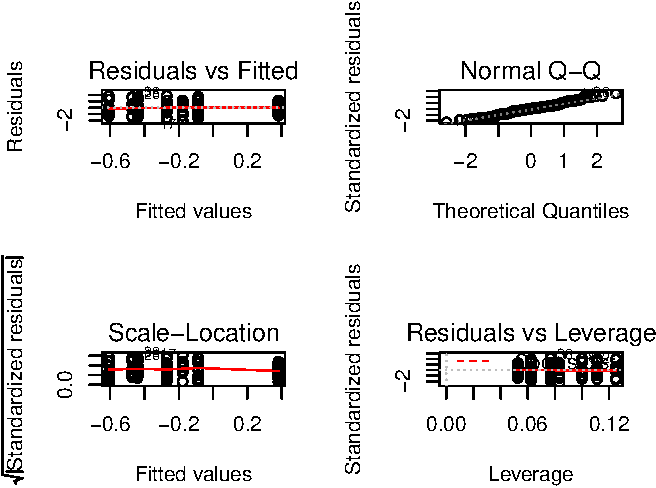
\includegraphics{04_BasicAnalyses_files/figure-beamer/unnamed-chunk-17-1.pdf}

\end{frame}

\begin{frame}[fragile]{Checking Assumptions}

They don't fit great on the slides but trust me that normality looks
good. The assumption of homogeneity of variance looks good as well.

But, if you wanted to test it, you could.

\begin{Shaded}
\begin{Highlighting}[]
\KeywordTok{library}\NormalTok{(car)}
\KeywordTok{leveneTest}\NormalTok{(fit2)}
\end{Highlighting}
\end{Shaded}

\begin{verbatim}
Levene's Test for Homogeneity of Variance (center = median)
      Df F value Pr(>F)
group  7   0.327 0.9399
      92               
\end{verbatim}

Large p-value here is a good thing: \texttt{emo::ji("smile")}
\footnote{This shows a smiley in `R`, just not on these slides---from the `emo` package on GitHub.}

\end{frame}

\section{Linear Regression}\label{linear-regression}

\begin{frame}{Linear Regression}

\large
Once again, linear regression is essentially the more flexible twin of
ANOVA and
t-tests.\footnote{It mainly only differs from ANOVA in the way it takes a dummy code rather than an effect code of the categorical variables.}

It can:

\begin{enumerate}
\def\labelenumi{\arabic{enumi}.}
\tightlist
\item
  Handle continuous and categorical predictors (i.e., independent
  variables)
\item
  Less stringent assumption of equality of variances
\item
  Is what many other methods are built on (Chapter 5 and 6 will talk
  about some of these)
\end{enumerate}

\end{frame}

\begin{frame}[fragile]{Linear Regression}

We will use \texttt{lm()} (Linear Model) to fit these models.

\small

\begin{Shaded}
\begin{Highlighting}[]
\NormalTok{fit5 =}\StringTok{ }\KeywordTok{lm}\NormalTok{(B }\OperatorTok{~}\StringTok{ }\NormalTok{A, }\DataTypeTok{data =}\NormalTok{ df)}
\KeywordTok{summary}\NormalTok{(fit5)}
\end{Highlighting}
\end{Shaded}

\begin{verbatim}

Call:
lm(formula = B ~ A, data = df)

Residuals:
    Min      1Q  Median      3Q     Max 
-1.9094 -0.6652  0.0356  0.6692  1.9487 

Coefficients:
            Estimate Std. Error t value Pr(>|t|)
(Intercept) -0.22050    0.13361  -1.650    0.102
A1           0.05337    0.18709   0.285    0.776

Residual standard error: 0.9352 on 98 degrees of freedom
Multiple R-squared:  0.0008298, Adjusted R-squared:  -0.009366 
F-statistic: 0.08139 on 1 and 98 DF,  p-value: 0.776
\end{verbatim}

\end{frame}

\begin{frame}[fragile]{Linear Regression}

We can add an interaction with the \texttt{*}. \small

\begin{Shaded}
\begin{Highlighting}[]
\NormalTok{fit6 =}\StringTok{ }\KeywordTok{lm}\NormalTok{(B }\OperatorTok{~}\StringTok{ }\NormalTok{A}\OperatorTok{*}\NormalTok{D, }\DataTypeTok{data =}\NormalTok{ df)}
\KeywordTok{summary}\NormalTok{(fit6)}
\end{Highlighting}
\end{Shaded}

\begin{verbatim}

Call:
lm(formula = B ~ A * D, data = df)

Residuals:
     Min       1Q   Median       3Q      Max 
-1.95215 -0.63769  0.00982  0.45819  2.22228 

Coefficients:
            Estimate Std. Error t value Pr(>|t|)
(Intercept) -0.27022    0.25141  -1.075    0.285
A1          -0.17046    0.35555  -0.479    0.633
D2           0.09247    0.36288   0.255    0.799
D3          -0.20133    0.40733  -0.494    0.622
D4           0.18359    0.33847   0.542    0.589
A1:D2       -0.09053    0.53497  -0.169    0.866
A1:D3        0.03429    0.55794   0.061    0.951
A1:D4        0.63770    0.47013   1.356    0.178

Residual standard error: 0.9065 on 92 degrees of freedom
Multiple R-squared:  0.1188,    Adjusted R-squared:  0.05178 
F-statistic: 1.772 on 7 and 92 DF,  p-value: 0.1023
\end{verbatim}

\end{frame}

\begin{frame}[fragile]{Other Specifications}

We can also make adjustments to the variables within the model.

First, we can transform the variables (e.g., log transformation).

\begin{Shaded}
\begin{Highlighting}[]
\NormalTok{fit7 =}\StringTok{ }\KeywordTok{lm}\NormalTok{(}\KeywordTok{log}\NormalTok{(B) }\OperatorTok{~}\StringTok{ }\NormalTok{A}\OperatorTok{*}\NormalTok{D, }\DataTypeTok{data =}\NormalTok{ df)}
\KeywordTok{summary}\NormalTok{(fit7)}
\end{Highlighting}
\end{Shaded}

We can change the reference level of a variable, too.

\begin{Shaded}
\begin{Highlighting}[]
\NormalTok{fit8 =}\StringTok{ }\KeywordTok{lm}\NormalTok{(B }\OperatorTok{~}\StringTok{ }\KeywordTok{relevel}\NormalTok{(D,}\DataTypeTok{ref =} \StringTok{"4"}\NormalTok{), }\DataTypeTok{data =}\NormalTok{ df)}
\KeywordTok{summary}\NormalTok{(fit8)}
\end{Highlighting}
\end{Shaded}

\end{frame}

\begin{frame}[fragile]{Checking Assumptions}

Assumption checking is similar to that of the linear model.

\begin{Shaded}
\begin{Highlighting}[]
\KeywordTok{par}\NormalTok{(}\DataTypeTok{mfrow =} \KeywordTok{c}\NormalTok{(}\DecValTok{2}\NormalTok{,}\DecValTok{2}\NormalTok{))}
\KeywordTok{plot}\NormalTok{(fit5)}
\end{Highlighting}
\end{Shaded}

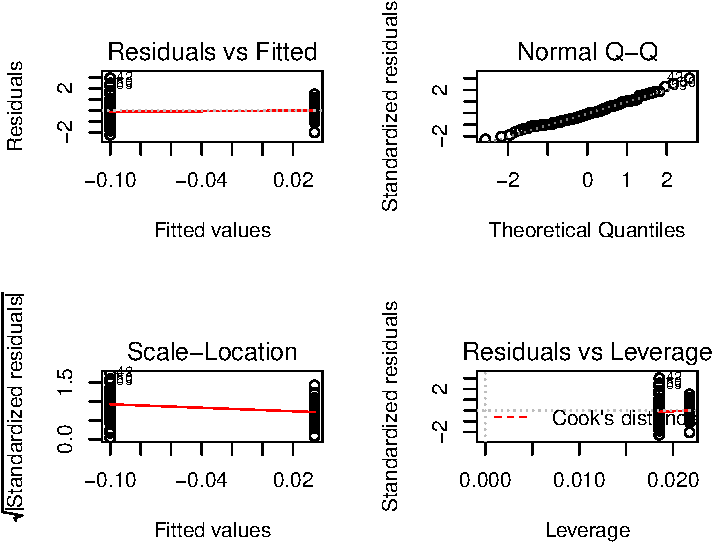
\includegraphics{04_BasicAnalyses_files/figure-beamer/unnamed-chunk-23-1.pdf}

\end{frame}

\section{Reporting Results}\label{reporting-results}

\begin{frame}[fragile]{Making This into a Table}

\Large
Often we want to present this information in a table. This can be done
is several ways:

\begin{enumerate}
\def\labelenumi{\arabic{enumi}.}
\tightlist
\item
  Pulling information out of the model objects directly
\item
  Using a package like \texttt{stargazer} to do that work for you
\item
  Manually by hand
\end{enumerate}

We can certainly do number 3 but why? So we'll look at both 1 and 2.

\end{frame}

\begin{frame}{Pull information out of the model objects}

The model objects contain loads of information that we can pull out:

\begin{enumerate}
\def\labelenumi{\arabic{enumi}.}
\tightlist
\item
  Coefficients
\item
  Standard Errors and P-values
\item
  Confidence Intervals
\item
  Fit Statistics
\item
  Predicted Values
\item
  and more! \footnote<.->{For a low cost of \$49.99! Kidding\ldots{}}
\end{enumerate}

\end{frame}

\begin{frame}[fragile]{Pull information out of the model objects}

To see what the model object holds: \small

\begin{Shaded}
\begin{Highlighting}[]
\KeywordTok{names}\NormalTok{(fit5)}
\end{Highlighting}
\end{Shaded}

\begin{verbatim}
 [1] "coefficients"  "residuals"     "effects"       "rank"         
 [5] "fitted.values" "assign"        "qr"            "df.residual"  
 [9] "contrasts"     "xlevels"       "call"          "terms"        
[13] "model"        
\end{verbatim}

\begin{Shaded}
\begin{Highlighting}[]
\KeywordTok{names}\NormalTok{(}\KeywordTok{summary}\NormalTok{(fit5))}
\end{Highlighting}
\end{Shaded}

\begin{verbatim}
 [1] "call"          "terms"         "residuals"     "coefficients" 
 [5] "aliased"       "sigma"         "df"            "r.squared"    
 [9] "adj.r.squared" "fstatistic"    "cov.unscaled" 
\end{verbatim}

\end{frame}

\begin{frame}[fragile]{Pull information out of the model objects}

\center
Using that information we can grab:

\begin{Shaded}
\begin{Highlighting}[]
\KeywordTok{summary}\NormalTok{(fit5)}\OperatorTok{$}\NormalTok{coefficients}
\end{Highlighting}
\end{Shaded}

\begin{verbatim}
               Estimate Std. Error    t value  Pr(>|t|)
(Intercept) -0.22049836  0.1336069 -1.6503519 0.1020725
A1           0.05337395  0.1870870  0.2852894 0.7760245
\end{verbatim}

or

\begin{Shaded}
\begin{Highlighting}[]
\KeywordTok{summary}\NormalTok{(fit5)}\OperatorTok{$}\NormalTok{fstatistic}
\end{Highlighting}
\end{Shaded}

\begin{verbatim}
      value       numdf       dendf 
 0.08139004  1.00000000 98.00000000 
\end{verbatim}

\end{frame}

\begin{frame}[fragile]{Pull information out of the model objects}

Put it in a table:

\begin{Shaded}
\begin{Highlighting}[]
\KeywordTok{rbind}\NormalTok{(}\KeywordTok{data.frame}\NormalTok{(}\KeywordTok{summary}\NormalTok{(fit5)}\OperatorTok{$}\NormalTok{coefficients, }\StringTok{"Type"}\NormalTok{=}\StringTok{"Simple Regression"}\NormalTok{),}
      \KeywordTok{data.frame}\NormalTok{(}\KeywordTok{summary}\NormalTok{(fit6)}\OperatorTok{$}\NormalTok{coefficients, }\StringTok{"Type"}\NormalTok{=}\StringTok{"Interaction"}\NormalTok{))}
\end{Highlighting}
\end{Shaded}

\begin{verbatim}
                Estimate Std..Error     t.value  Pr...t..
(Intercept)  -0.22049836  0.1336069 -1.65035186 0.1020725
A1            0.05337395  0.1870870  0.28528939 0.7760245
(Intercept)1 -0.27022085  0.2514114 -1.07481545 0.2852682
A11          -0.17046286  0.3555494 -0.47943510 0.6327669
D2            0.09247451  0.3628811  0.25483418 0.7994200
D3           -0.20133155  0.4073330 -0.49426771 0.6222953
D4            0.18358504  0.3384729  0.54239206 0.5888599
A1:D2        -0.09052975  0.5349676 -0.16922472 0.8659914
A1:D3         0.03429375  0.5579407  0.06146485 0.9511223
A1:D4         0.63769917  0.4701266  1.35644146 0.1782782
                          Type
(Intercept)  Simple Regression
A1           Simple Regression
(Intercept)1       Interaction
A11                Interaction
D2                 Interaction
D3                 Interaction
D4                 Interaction
A1:D2              Interaction
A1:D3              Interaction
A1:D4              Interaction
\end{verbatim}

\end{frame}

\begin{frame}[fragile]{Pull information out of the model objects}

\Large
On the previous slide we:

\begin{enumerate}
\def\labelenumi{\arabic{enumi}.}
\tightlist
\item
  Created two \texttt{data.frame} with the coefficients and a variable
  called \texttt{"Type"}
\item
  Glued them together by row with \texttt{rbind()}
\end{enumerate}

This is a simple way of putting a table together that you can later
export.

\end{frame}

\begin{frame}[fragile]{Use a package like \texttt{stargazer} to do that
work for you}

A simpler but less flexible way is using a package like
\texttt{stargazer}. \tiny

\begin{Shaded}
\begin{Highlighting}[]
\KeywordTok{library}\NormalTok{(stargazer)}
\KeywordTok{stargazer}\NormalTok{(fit5, fit6, }\DataTypeTok{type =} \StringTok{"text"}\NormalTok{)}
\end{Highlighting}
\end{Shaded}

\begin{verbatim}

=========================================================
                             Dependent variable:         
                    -------------------------------------
                                      B                  
                           (1)                (2)        
---------------------------------------------------------
A1                        0.053              -0.170      
                         (0.187)            (0.356)      
                                                         
D2                                           0.092       
                                            (0.363)      
                                                         
D3                                           -0.201      
                                            (0.407)      
                                                         
D4                                           0.184       
                                            (0.338)      
                                                         
A1:D2                                        -0.091      
                                            (0.535)      
                                                         
A1:D3                                        0.034       
                                            (0.558)      
                                                         
A1:D4                                        0.638       
                                            (0.470)      
                                                         
Constant                  -0.220             -0.270      
                         (0.134)            (0.251)      
                                                         
---------------------------------------------------------
Observations               100                100        
R2                        0.001              0.119       
Adjusted R2               -0.009             0.052       
Residual Std. Error  0.935 (df = 98)    0.906 (df = 92)  
F Statistic         0.081 (df = 1; 98) 1.772 (df = 7; 92)
=========================================================
Note:                         *p<0.1; **p<0.05; ***p<0.01
\end{verbatim}

\end{frame}

\begin{frame}[fragile]{Use a package like \texttt{stargazer} to do that
work for you}

This particular package can take several model objects and produce a
nice table. It is hard to see but it includes the number of
observations, fit statistics, the coefficients, and f-statistics.

Other packages exist that do similar things (e.g., \texttt{texreg}).

\begin{Shaded}
\begin{Highlighting}[]
\KeywordTok{library}\NormalTok{(texreg)}
\KeywordTok{screenreg}\NormalTok{(}\KeywordTok{list}\NormalTok{(fit5, fit6))}
\end{Highlighting}
\end{Shaded}

\end{frame}

\section{Conclusions}\label{conclusions}

\begin{frame}{Conclusion}

\Large

\begin{enumerate}
\item Performing linear models is straightforward in `R`
\item With a few lines of code, we can fit a model and check model assumptions
\item We can easily turn our model information into an informative table
\end{enumerate}

\end{frame}

\begin{frame}

\centerline{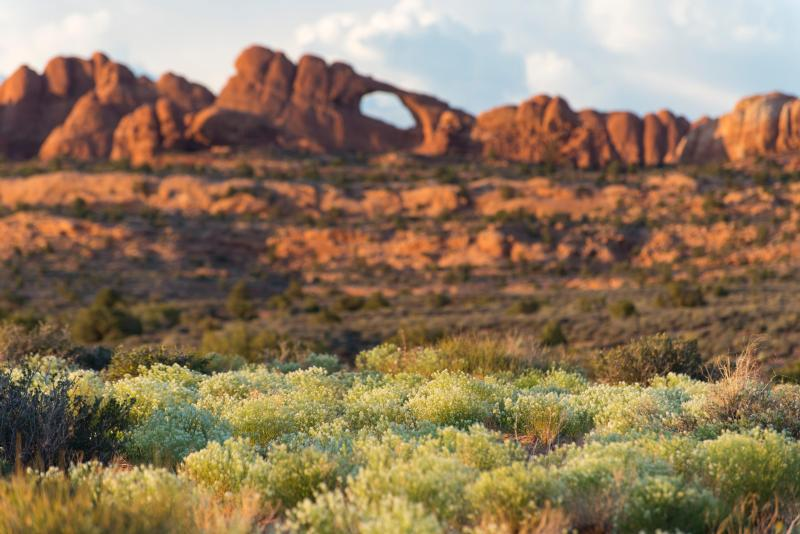
\includegraphics[height=7in]{Figures/grass_landscape_arch.jpg}}

\end{frame}
